\documentclass[11pt, twocolumn]{article}

\usepackage[T1]{fontenc}
\usepackage[utf8]{inputenc}
\usepackage{indentfirst}		% pacchetto per avere il rientro anche nella prima riga di una sezione
\usepackage{courier}		% pacchetto per usare il font Courier per i piccoli pezzi di codice o i nomi dei file
\usepackage{amsfonts}
\usepackage{amsmath}		% pacchetto per equazioni
\usepackage{amsthm}		% pacchetto per i teoremi, da dichiarare DOPO amsmath!
\usepackage{amssymb}		% pacchetto per insiemi matematici
\usepackage[english]{babel}		% scelgo l'inglese come lingua
\usepackage{verbatim}	% pacchetto per i commenti in blocco
\usepackage{graphicx}% pacchetto per le immagini
\usepackage{subfigure}% pacchetto per le immagini raggruppate
\usepackage{fancyhdr}% Pacchetto per header personalizzati
\usepackage{float}	% lo uso per mettere le immagini dove voglio con H

\topmargin=-0.45in
\evensidemargin=0in
\oddsidemargin=0in
\textwidth=6.5in
\textheight=9.0in
\headsep=0.25in 
\linespread{1.1}	% spazio tra le linee


\newcommand{\hmwkAuthorName}{Tommaso Martini - 1081580}
\lhead{LZ77 and LZSS Algorithms} % Top left header
\rhead{\hmwkAuthorName} % Top right header

\begin{document}

\title{{\Large Source Coding - Final Project} \\ \textsc{\LARGE \textbf{The LZ77 and LZSS Algorithms for Data Compression}}}
\date{July 25, 2014}
\author{Tommaso Martini (108 15 80)}
        
\maketitle

\section{Introduction}
This final project has the aim of developing a dictionary-based compression coding technique and comparing the gained performances with those of softwares present in a typical PC. In particular, we are required to develop our own version of the LZ77 and LZSS algorithms.

In the following we will give a brief overview of such algorithms and we will explain how our versions have been implemented, focusing on the implementation choices. Eventually, we will provide a comparison between the two algorithms and their commercial versions, when they work to compress several kinds of file.

The last section gathers all the further developments which would complete or improve the performances of our implementation.

\subsection{Dictionary-based coding} \label{subsec:dict-base}
A \textit{dictionary-based coding} is a coding technique which processes a file as a sequence of symbols to build a dictionary, that is a sequence of pairs (key, value), where the value can be either a symbol or a sequence itself. The dictionary, properly formatted, is the message to send to the receiver. The latter has to build back the original sequence exploiting the information contained in the dictionary entries. Actually, for the dictionaries we will be using, we do not care very much about the keys, since the entries are stacked with the same order the receiver will use at its side, therefore we will not talk about a key for a dictionary entry, rather than about a position.

There are two kinds of dictionary-based coding technique, depending on the dictionary form. The first is the \textit{implicit dictionary coding}, which is the case of the LZ77 algorithm, in which the entries are generated and read sequentially, without the need of specifying a key for them. On the other hand, the \textit{explicit dictionary coding} creates some entries which are referred to with their keys and, in the decoding process, are used also non-sequentially. This is the case of the LZ78 algorithm, published by the same authors of the LZ77 one year later.





\section{The LZ77 Algorithm} \label{sec:lz77}
In this section we provide a short overview of the dictionary-based compression algorithm presented by Abrham Lempel and Jacob Ziv in 1977 \cite{ziv1}. The aim of this algorithm is trying to reduce the redundancy due to similar sequence repeating along the message. What it does is basically checking if a certain piece of the sequence has already been found in the past and, if it is the case, we code the whole piece with a reference to the previous alike sequence.

\subsection{The algorithm} \label{subsec:lz77alg}
The algorithm works with two adjacent windows shifting on the right during the coding of the message. The first window is the \textit{searching window} and has length $L_s$; the second one is the \textit{coding window} and has length $L_c$. We want to find a match between any prefix of the \textit{coding window} and a sequence contained in the overall window given by the juxtapposition of the \textit{searching window} and the \textit{coding window}, i.e. it is sufficient that only the first symbol of the match belongs to the \textit{searching window}, while the matched pattern can stretch in through the \textit{coding window} itself. The window lengths $L_s$ and $L_c$ are two parameters of the algorithm and their choice strongly influences the compression performances, we will see how in the last part of this report.
 
Once we have found a match between a prefix of the \textit{coding window} and another piece of message, we code it as a triplet (\textit{offset}, \textit{length}, \textit{symbol}) where:
\begin{itemize}
\item
\textbf{offset} denotes the number of back hops we have to do, starting from the first symbol of the \textit{coding sequence}, to find the beginning of the matched string; it is clear that, for how it is defined, the \textit{offset} cannot exceeds the \textit{searching window} dimension;

\item
\textbf{length} is the length of the matched string or, equivalently, of the prefix of the \textit{coding window} which has been matched. This value cannot exceed $L_c$, since this is the maximum dimension of the pattern we are looking for;

\item
\textbf{symbol} is the first symbol after the matched prefix of the \textit{coding window}. Its encoding assures the functioning of the algorithm also in case of no matches. 
\end{itemize}

After the generation and the storage of a triplet inside the dictionary, we shift the windows such that the first symbol of the \textit{coding window} corresponds to the first non encoded symbol.

\subsection{LZ77 Implementation} \label{subsec:lz77implem}
In the following paragraphs we will present our own implementation in Matlab of the algorithm, spanning the different versions we produced. As a matter of fact, several editions of the same program have been written, adopting different approaches in some parts of the code. Actually the versions differ above all for the pattern matching algorithm that has been adopted, while the rest of the code remains basically the same.

\subsubsection{Basic Coding Algorithm} \label{subsubsec:basiclz77}
First of all we choose a file and write it as a sequence of bytes (\texttt{uint8} in Matlab). We assume this is the original message, whose alphabet is made of all the possible combinations of $8$ bits and has size $M = 2^8 = 256$. The first symbol of the sequence is encoded as a single symbol directly, because placing the \textit{coding window} in the first positions makes no sense, since we would have no \textit{searching window} to exploit. Then, the \textit{coding window} starts from the second position of the sequence and, until there are at least $L_s$ symbols before it, the \textit{searching window} is shrunk to fit into the available positions. The same thing happens to the \textit{coding window} when we are reaching the end of the file: if less than $L_c$ symbols are left, we use a shorter \textit{coding window}. Note that, in order to always have a symbol to insert in the \textit{symbol} field of the last triplet, near the end of the file the \textit{coding window} is shrunk such that the last symbol of the stream is left out.

Once the dictionary has been created, we want to write it using the least amount of memory we can. Since the values of $L_s$ and $L_c$ are fixed and determine the maximum values for the fields \textit{offset} and \textit{length} and we know that a symbol is represented with a single byte, we can evaluate the maximum number of bits to use for each triplet as:
\begin{align}
l_{offset} &= \left \lceil log_2L_s \right \rceil \text{bits} \\
l_{length} &= \left \lceil log_2L_c \right \rceil \text{bits} 
\end{align}

We use exactly $l_{offset} + l_{length} + 8$ bits for each triplet. Once we have created a sequence of bits by lining up all the rows of the dictionary, we can split it in blocks of $8$ bits and code it as a sequence of bytes. To let the receiver know how many bits represent each element of the triplet, we attach in front of the stream three bytes: the first indicating the number of bits related to the \textit{offset}, the second related to the \textit{lenght} and the third to the \textit{symbol}. One may argue that, with a single byte, we can referring only to values smaller than $2^8 = 256$; this is true, but, for our purposes, a byte is more than sufficient: suppose we need $200$ bits to represent the \textit{offset} in a triplet; this means that our \textit{searching window} is almost $2^{200}$ bits long, that is around $2 \times 10^{50}$ Gigabytes, of course absolutely useless for ordinary files. At the receiver side the user inspects the first three bytes to retrieve the number of bits dedicated to each component of the triplet. Then, after looking at the message as a stream of bits, it can group together the triplets of the dictionary by exploiting the information just got. This explains also why we cannot use less than $3$ bytes to express the dimension of one triplet: since the \textit{byte} is the fundamental unity of memory in every computer, we are sure that every user is able to get the initial information and thus decoding the dictionary. 

\subsubsection{Version 1: Basic}
As previously mentioned, the several versions of the algorithms differ by the pattern matching technique to find the \textit{coding window} inside the \textit{searching window}. The first, basic, version of the program executes the pattern matching by brute force: we compare the first character of the \textit{coding window} with each element of the \textit{search window}. When a match occurs, we compare the second element of the \textit{coding window} with the following symbol of the \textit{search window} and so on until we find two different symbols. Then, if the length of the match is larger than the longest match found so far, we replace it and save also the starting point of the match in the \textit{search window}. If, in the end, the longest match has zero length, this means that no match has been found and we have to encode one only symbol. This basic algorithm is very wasteful, because we have to try every possible position.

\subsubsection{Version 2: KMP}
A first improvement has been brought by using the KMP (Knuth-Morris-Pratt) pattern mathcing algorithm \cite{knuth1}. This algorithm is optimum for the research of a pattern inside a string: it takes a time $\mathcal{O}(n + k)$, where $n$ is the length of the pattern and $k$ is the length of the string. We though about using the KMP algorithm where the pattern $\mathbf{c}$ is the \textit{coding window} and the overall string $[\mathbf{s}, \mathbf{c}]$ is the \textit{search window} concatenated with the \textit{coding window}.

The KMP algorithm starts with the brute force approach, comparing the first character of the pattern with each character of the string, but it allows to improve performances in pattern matching because, thanks to previous failed matches, it realizes when it is possible to jump ahead and discard some trials, which will surely fail. We used the "jump mechanism" of KMP to realize a second version of the program, but the time performances keep remaining very poor, due to the many nested cycles we have to use, which are not very fast to be executed in Matlab. Moreover, each different pattern needs a \textit{matching function} to be computed, which increases the number of necessary computations.

\subsubsection{Version 3: optimistic \texttt{strfind()}}
The third version uses the Matlab function \texttt{strfind()} for pattern matching, which is optimized to work in Matlab. We simply invoke this method using the \textit{search window} as string and the \textit{coding window} as pattern to be found. If no matches occurs we discard the last symbol of the \textit{coding window} and repeat the procedure until either a match is found or we reduce the length of the pattern to zero, that means that we have to encode the symbol individually.

The term \textit{optimistic} refers to the order in which we take different patterns: we are confident to find the longest match, the best one, quite soon and therefore we start by looking for the entire pattern. Of course, if there is little redundancy and there is often no match found, we have to repeat the cycle $L_c$ times for each different \textit{coding window}.

\subsubsection{Version 4: pessimistic \texttt{strfind()}} \label{subsubsec:pess}
From an empirical point of view we found that we often have not many long matches and hence the \textit{optimistic} approach is not very suitable. The \textit{pessimistic} approach consists in starting to look for a match with the shortest possible prefix of the \textit{coding window} and executing the pattern matching through \texttt{strfind()} until we find no more matches. In this case we consider the previous match, which is the longest one, to build the current triplet. If there are no matches we know it from the first iteration and this allows us to save a lot of time. Quite all the results presented in the following have been obtained with this version of the program.

\section{The LZSS Algorithm}
The LZ77 algorithm has a lack of performances due to the constraint on the triplet to send: whenever we have to encode a single symbol, we have to waste $l_{offset} + l_{length}$ bytes because the \textit{offset} and the \textit{length} of the match are both zero. In fact the triplet to send is $[0, 0, \alpha]$. In 1982 Storer and Szymanski \cite{storer1} proposed a different version of the LZ77 algorithm which improves the compression performances through a better management of the size of the dictionary entries.

We can distinguish two kinds of entries: those which contain the information related to an only symbol not find in the \textit{search window} and those which refer to a previous pattern. We can use a flag bit to indicate in which case we are. If the bit is $0$ the entry is made only by the code of a symbol. If the bit is $1$ the entry is made of a pair (\textit{offset}, \textit{length}). This convention allows us to save a lot of space in memory in both cases.

\subsection{LZSS Implementation}
The main difference with the LZ77 implementation lies on the dictionary construction, all the rest of the code is quite the same used in in the version $4$ of the LZ77 exposed in section \ref{subsubsec:pess}, with a pessimistic usage of the function \texttt{strfind()} for pattern matching.

The problem with the usage of flag bits is that every computer works with bytes as fundamental memory unit. Since we cannot simply add a surplus bit to each sequence of bytes forming a dictionary entries, we decided to spend a whole byte to gather the flags for $8$ consecutive entries. The sequence of these $8$ bits is read as a only value and is transmitted as part of the message in front of the entries it is referring to. At the receiver side the knowledge of the number of bytes used to encode \textit{offset}, \textit{length} and \textit{symbol} fields allows a unique interpretation of the message. Once the receiver has build the dictionary, it can proceed with the reconstruction of the original message.

\section{Performances of the Algorithms}
We want now to focus our attention on the performances reached by our implementations of the LZ77 and LZSS algorithms in relation both with the type of file we are trying to compress and the parameters setting, that is the lengths of the \textit{searching window} and the \textit{coding window}.

\subsection{Testing files}
All the experiments we performed have been executed on seven specific types of files, part of them taken from the \textit{Canterbury Corpus}, a collection of files with several formats to be used as sample files for compression testing. The used files are here reported:

\begin{itemize}
\item
\textbf{\texttt{rep.txt}}: simple text file containing a sequence of character \texttt{A} repeated $10000$ times ($10000$ bytes);

\item
\textbf{\texttt{per}}: file containing $10$ repetitions of a random sequence of $1000$ bytes ($10000$ bytes);

\item
\textbf{\texttt{ran}}: file generated by concatening $10000$ random bytes ($10000$ bytes);

\item
\textbf{\texttt{shak.txt}}: simple text file reporting a piece of a Shakespeare poem ($13741$ bytes);

\item
\textbf{\texttt{web.html}}: html format page ($24603$ bytes);

\item
\textbf{\texttt{code.c}}: piece of \texttt{c} code ($11150$ bytes);

\item
\textbf{\texttt{sum}}: SPARC executable file ($38240$ bytes).
\end{itemize}

We chose these files to have a wide span among different kinds of files and show, in this way, the several behaviours the algorithm can assume for different scenarios. In particular, we use the file \texttt{rep.txt} to obtain the maximum compression capability of the algorithm, the file \texttt{per} was included to show the behaviours in presence of periodicity and the file \texttt{ran} represents the worst scenario for compression purposes, since it has no redundancy to exploit and a high entropy. The last four files, on the other hand, do not represent borderline or special cases, but more common examples of files one can deal with during his ordinary life.

\subsection{Redundant file}
The first file, \texttt{rep.txt}, is the most redundant file we can have: $10000$ repetitions of the same character, \texttt{A}. The nature of the file allows a very strong compression, since we could just say what is the symbol and how many times it is repeated. The following table shows the performances of the algorithms executed with a fixed \textit{coding window} of length $2000$ and a \textit{searching window} varying between $1000$, $5000$ and $10000$, which is the length of the message itself:
\begin{center}
\begin{tabular}{r | c | c |}
\multicolumn{3}{c |}{\texttt{rep.txt}} \\ \hline
$L_s$ & LZ77 & LZSS \\ \hline
1000 & $0.25$\% & $0.19$\% \\
5000& $0.27$\% & $0.20$\% \\
10000& $0.28$\% & $0.21$\% \\
\hline
\end{tabular}
\end{center}

As we expected the compression is very high: we can represent $10000$ bytes with less than $30$ bytes. It may look strange that performances drop with the increasing of the \textit{searching window}; this is due to the number of bits we need to encode a triplet, which raises with the length of the window (in LZ77 we use $29$ bits when $L_s = 1000$, $32$ bits when $L_s = 5000$ and $35$ bits when $L_s = 1000$). LZSS works to solve this issue, as a matter of fact it behaves slightly better than LZ77 and manages to encode the dictionary with less bits. In this case we can see that the length of the \textit{coding window} has also a great relevance on performances; the followig table summarizes the results obtained when we use the same three searching lengths of the previous example, but a coding length $L_c = 10000$:
\begin{center}
\begin{tabular}{r | c | c |}
\multicolumn{3}{c |}{\texttt{rep.txt}} \\ \hline
$L_s$ & LZ77 & LZSS \\ \hline
1000 & $0.11$\% & $0.08$\% \\
5000& $0.22$\% & $0.08$\% \\
10000& $0.12$\% & $0.09$\% \\
\hline
\end{tabular}
\end{center}
In this case we just need about ten bytes to represent the whole message and the dictionary is composed by only two rows.
It is interesting to report here the 3D plot of the LZ77 performances, in percentage of compression, in function of $L_s$ and $L_c$:

\begin{center}
\begin{figure}[H]
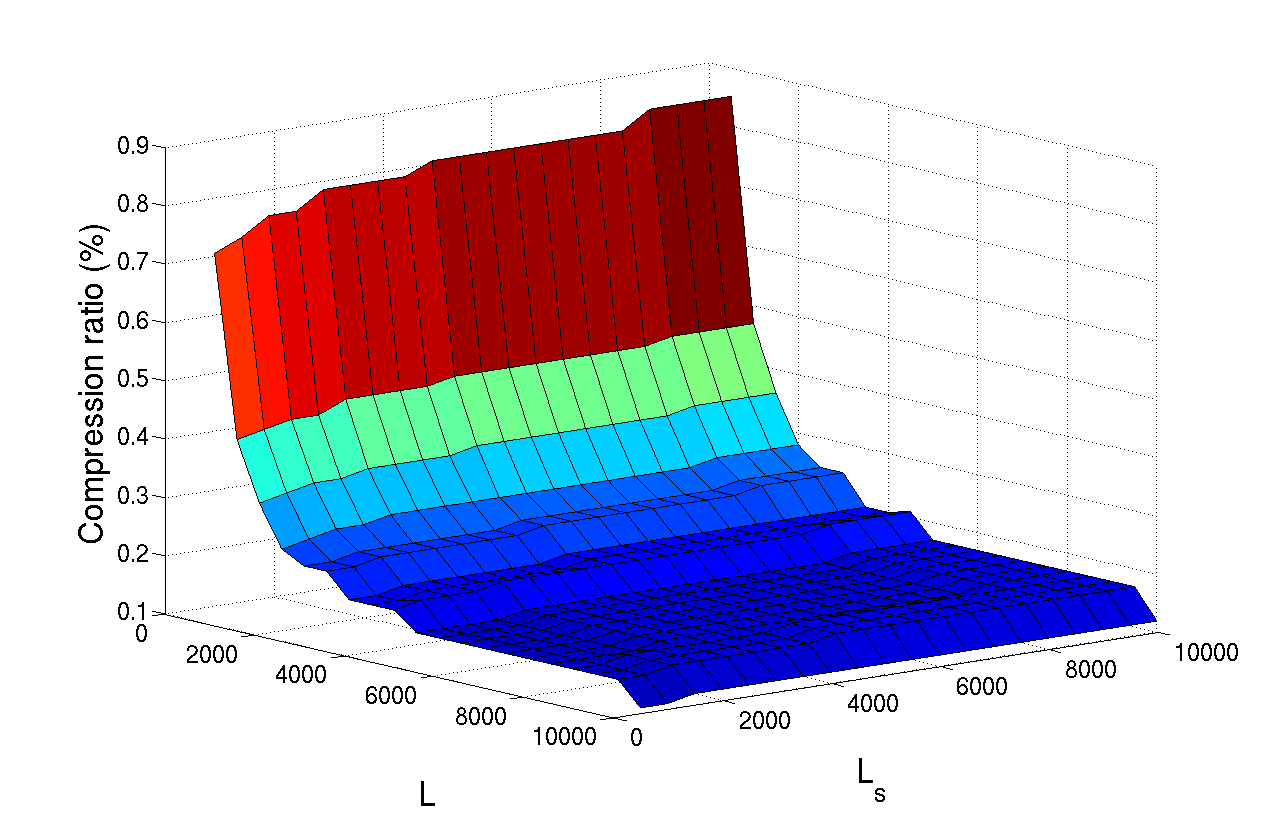
\includegraphics[width=8.5cm]{images/rep_surf.png}
\caption{LZ77 compression ratio in function of $L_s$ and $L_c$.}
\end{figure}
\end{center}

The above plot well shows that for this file the choice of the \textit{coding window} is more important than the choice of the \textit{searching window}, which, we will see, is not common for a generic file.

\subsection{Periodic file}
A big problem with implicit dictionary based compression algorithms is that periodicity of the message could not be properly exploited. This unfavorable event occurs if the windows are shorter than the period of the message, such that there is no way the algorithm can become aware of the existance of periodicity in the message; the LZ78 algorithm was born to solve this issue. We can bring a clear example compressing the file \texttt{per} keeping fixed the \textit{coding window} to $2000$, but with two different \textit{searching window} lengths: $500$ (half a period) and $5000$ (five times a period). The compression results are reported in the following table:

\begin{center}
\begin{tabular}{r | c | c |}
\multicolumn{3}{c |}{\texttt{per}} \\ \hline
$L_s$ & LZ77 & LZSS \\ \hline
500 & $189.98$\% & $112.53$\% \\
5000& $23.55$\% & $11.44$\% \\
\hline
\end{tabular}
\end{center}

It is clear that, in the first case, the algorithm is not exploiting the periodicity, in fact it is expanding the data and increasing the file dimension, because, being the period built randomly, it finds no redundancy to exploit. In the second scenario, however, periodicity is exploited and the file is strongly compressed.

\subsection{Randomly generated file}
When a file is made by a random sequence of bytes its entropy is very high and the algorithm finds no redundancy to exploit for compression. In this case performances are very low, in fact the output file has a greater dimension than the input file and we can do very little also by varying $L_s$ and $L_c$. The following table reports the compression ratios with $L_c = 2000$ and $L_s = 1000, \ 5000, \ 10000$:

\begin{center}
\begin{tabular}{r | c | c |}
\multicolumn{3}{c |}{\texttt{ran}} \\ \hline
$L_s$ & LZ77 & LZSS \\ \hline
1000 & $184.66$\% & $112.53$\% \\
5000& $197.83$\% & $112.55$\% \\
10000& $202.12$\% & $112.56$\% \\
\hline
\end{tabular}
\end{center}

We can notice two main facts: the first is that LZSS compresses in general better than LZ77; the second is that LZSS performances decrease much more slowly than LZ77; if we inspect the dictionaries created by the two algorithms, we can try to spot the reason of such difference: the LZ77 dictionary contains a lot of references to an only previous symbol and we cannot avoid using a whole triplet to encode them. On the other hand the LZSS algorithm is able to realize that it is not a good deal to waste a whole triplet to express an only symbol and it encodes it as a single byte. In this way we ideally would have a dictionary with the same dimensions of the message, but, unlucklily, the coding algorithm also includes the flag bits. Thus, it is practically quite impossible to compress a random sequence: if we try to compress it, we are going to hopelessly expand it.

\subsection{Common files}
The file \texttt{shak.txt} is an example of human-written text file. As we can see from the results of the experiment, LZ77 and LZSS are not the best choice for compressing this kind of file. The reason is that the spoken language has not a strong redundancy and patterns of characters are often short and repeated only a few times. The table below shows the performances with $L_c = 2000$:
\begin{center}
\begin{tabular}{r | c | c |}
\multicolumn{3}{c|}{\texttt{shak.txt}} \\ 
\hline
$L_s$ & LZ77 & LZSS \\ \hline
1000 & $89.48$\% & $77.91$\% \\
5000& $82.26$\% & $72.52$\% \\
10000& $81.38$\% & $71.93$\% \\
\hline
\end{tabular}
\end{center}

Code files as \texttt{web.html} and \texttt{code.c} presents a greater redundancy because of their scientific format; strict rules of the programming languages make them very repetitive and thus the LZ77 and the LZSS manage to perform a better compression of such files. The following tables show the results for the two files where a $2000$ symbols long \textit{coding window} has been used:
\begin{center}
\begin{tabular}{r | c | c |}
\multicolumn{3}{c|}{\texttt{code.c}} \\
\hline
$L_s$ & LZ77 & LZSS \\ \hline
1000 & $73.53$\% & $59.72$\% \\
5000& $62.25$\% & $52.98$\% \\
10000& $58.68$\% & $50.14$\% \\
\hline
\end{tabular}

\vspace{0.5cm}

\begin{tabular}{r | c | c |}
\multicolumn{3}{c|}{\texttt{web.html}} \\
\hline
$L_s$ & LZ77 & LZSS \\ \hline
1000 & $59.82$\% & $49.27$\% \\
5000& $51.65$\% & $43.02$\% \\
10000& $51.45$\% & $42.93$\% \\
\hline
\end{tabular}
\end{center}

The executable file \texttt{sum} can also be quite well compressed:
\begin{center}
\begin{tabular}{r | c | c |}
\multicolumn{3}{c|}{\texttt{sum}} \\ 
\hline
$L_s$ & LZ77 & LZSS \\ \hline
1000 & $68.91$\% & $60.58$\% \\
5000& $61.85$\% & $56.70$\% \\
10000& $55.83$\% & $51.61$\% \\
\hline
\end{tabular}
\end{center}

To conclude this section it is interesting to plot a surface graph of the performances in function of both $L_s$ and $L_c$. We compressed files \texttt{shak.txt} and \texttt{code.c} changing both the \textit{searching window} and the \textit{coding window} from $L_s = L_c = 1000$ to the dimension of the files themselves, with step of $1000$. Note that, if the windows are larger than the file sizes, it makes no difference how large the buffers are, because the windows are shrunk to adapt to the actual length of the message.

\begin{center}
\begin{figure}[H]
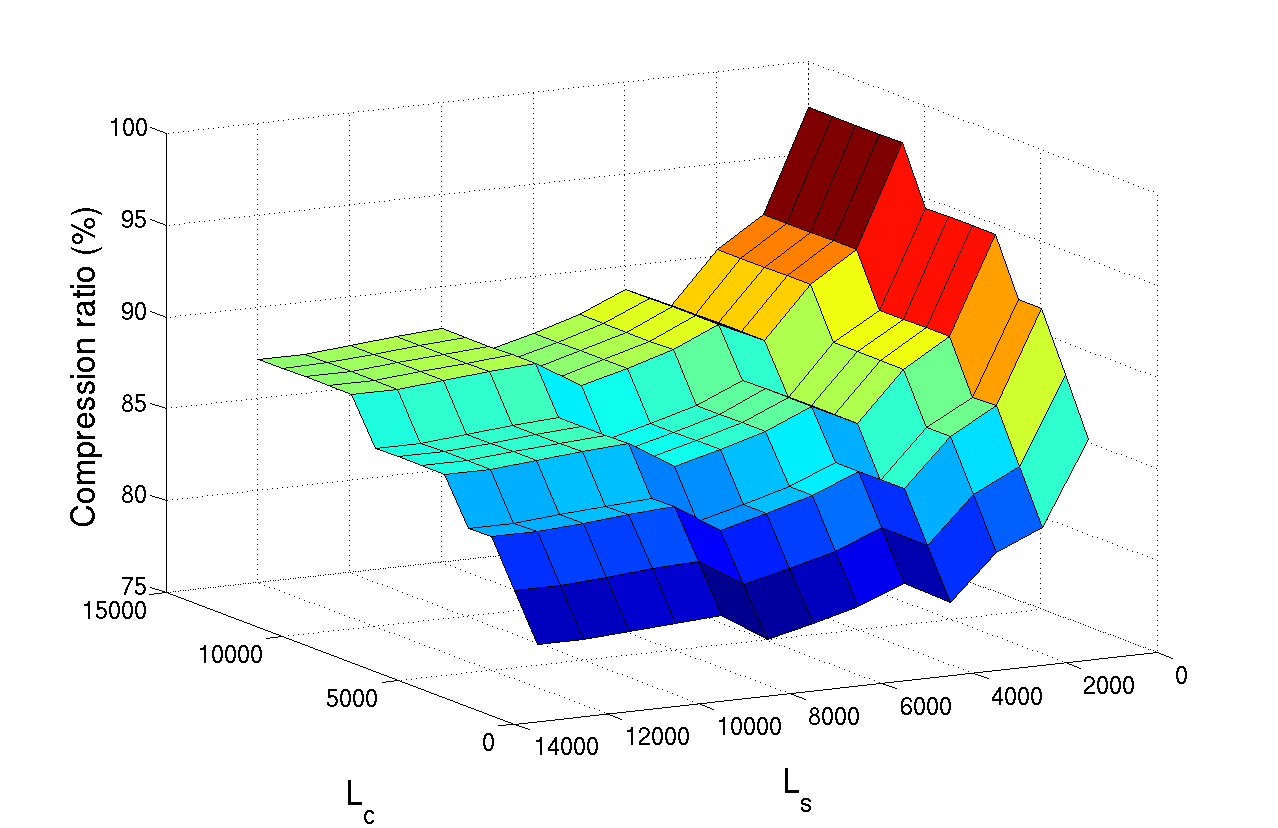
\includegraphics[width=8.5cm]{images/lz77_4.png}
\caption{LZ77 compression ratio for \texttt{shak.txt}.}
\end{figure}
\end{center}

\begin{center}
\begin{figure}[H]
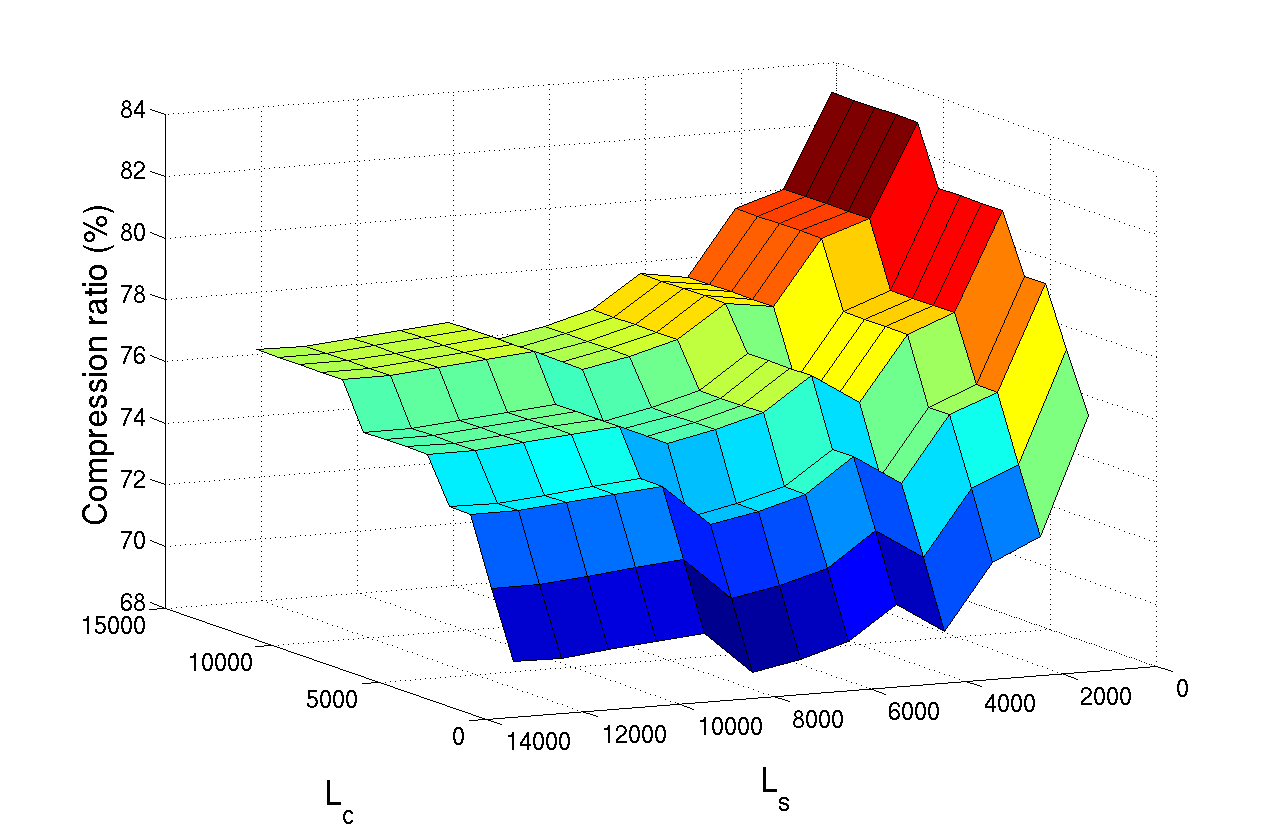
\includegraphics[width=8.5cm]{images/lzss_4.png}
\caption{LZSS compression ratio for \texttt{shak.txt}.}
\end{figure}
\end{center}

\begin{center}
\begin{figure}[H]
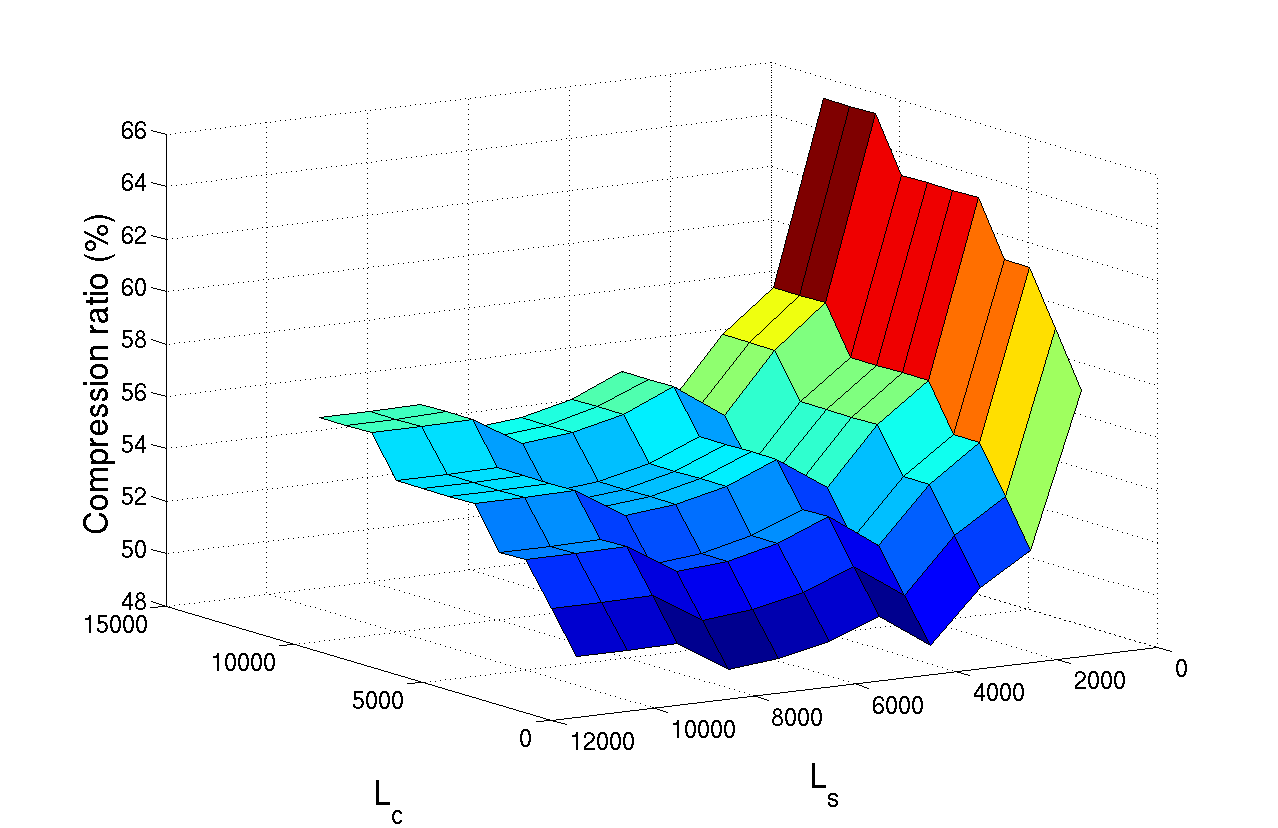
\includegraphics[width=8.5cm]{images/lz77_6.png}
\caption{LZ77 compression ratio for \texttt{code.c}.}
\end{figure}
\end{center}

\begin{center}
\begin{figure}[H]
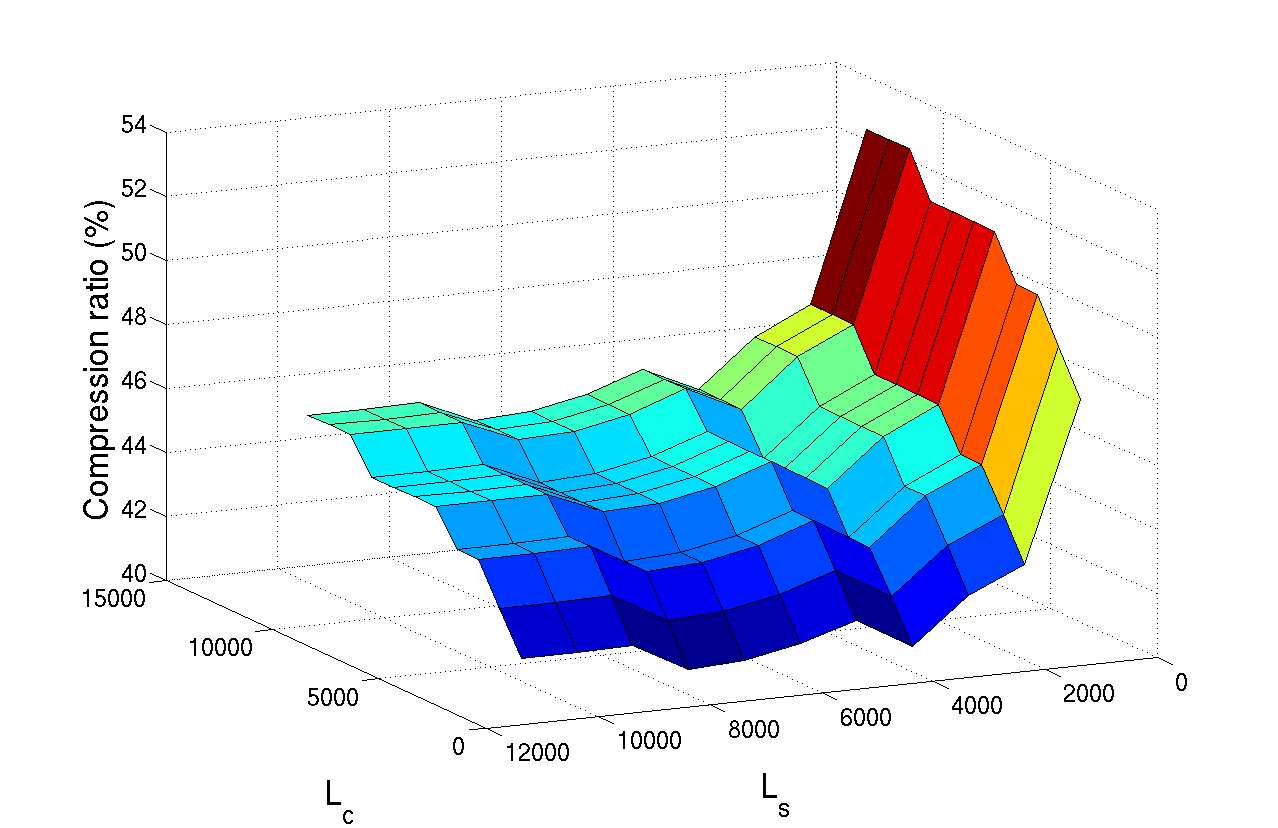
\includegraphics[width=8.5cm]{images/lzss_6.png}
\caption{LZSS compression ratio for \texttt{code.c}.}
\end{figure}
\end{center}

Two main things can be noticed from the above graphs. First of all we have a confirmation that the LZSS works in general better than the LZ77, as a matter of fact plots related to the LZSS lie below the corresponding LZ77 plots. The second, and most relevant information, links the window sizes with the compression performances: it is intuitive that large \textit{searching windows} are more suitable, because, if we consider a long sequence of symbols, finding some repeated patterns is more likely; on the other hand, and this could be less intuitive, increasing the \textit{coding window} is not very advisable: it is clear that a too short \textit{coding window} is not a good deal, because we risk to encode a unique, long pattern with more pairs (\textit{offset}, \textit{length}) than necessary. But why should enlarging it be even worse? The reason is that, in common files as the ones we used for the experience, repeated patterns are never very long, therefore having a huge \textit{coding window} does not represent a profit, in fact we need many bits to represent the \textit{length} field. To conclude, even though performances depend on the kind of file we are trying to compress, we should prefer a quite short \textit{coding window} and a large \textit{searching window}, being careful that this choice may affect time performances.


%It is easy to see that performances tends to improve with the growing of the \textit{searching window}. We could expect such a result: with shorter windows it is more difficult to find repeated pattern to refer to and, in some cases, we could neither realize that such patterns are present in the message. For a highly redundant input stream a long window allows to encode at the same time much more repetitions; even though the number of bits needed to represent a wide range of values grows with the increasing of the window, this happens with a logarithmic trend, while the amount of space used to encode a sequence byte per byte grows linearly. Clearly the usage of large windows implies a drop of performances from a computational time point of view. 
%In the best compression scenario, we would like to have a \textit{search window} as long as the message itself, but, since this is not suitable for time reason, commercial softwares usually work with block of symbols $32$ Kbyte long with windows of


\section{Comparison with existing softwares}
In this section we report some results obtained by the comparison between our implementations and other softwares usually installed in common PCs. We want to mention right now that our implementations have no chances to behave as well as any of the professional softwares employed by default by a PC. The reasons are mainly two: the first one is that programs that compress files or folders into archives .ZIP use an advanced algorithm, where the simple LZ77 is enhanced by further coding, in particular by a Huffman code; this combined coding is called LZ77 Deflate, is used by most of the .ZIP compressors and will be shortly described in the following. The second reason is about time: since we execute our program in Matlab, performances are lowered by the infrastructure of the environment and, moreover, \texttt{for} cycles are not very convenient in this particular language. 

\subsection{LZ77 Deflate}
The \textit{deflate} algorithm differs from the simple LZ77 for the final compression of the dictionary through a Huffman code. The description of the basic version of the algorithm can be found in the RFC1951 \cite{deut1}, here we provide only a brief overview of its functioning.
\\

The original file is first split into blocks of data whose maximum length must be $64$ Kbytes. The LZ77 dictionary is generated through the known procedure, with $L_s = 32000$ and $L_c = 258$ bytes. Once the dictionary is generated, it is compressed using a Huffman code; even if we have three types of data to express (\textit{symbol}, \textit{offset} and \textit{length}), we use only two Huffman trees. The first tree is made of $285$ codewords: the first $256$ ($0, \ldots, 255$) stand for literals, that is the symbols (we look at the message as a sequence of bytes), value $256$ indicates the end of the block of data and values $257, \ldots, 285$ are used to indicate the \textit{length} field, which can assume values in $0, \ldots, 258$. Note that some of the \textit{length} codewords are used to represent more than one actual length, for example value $277$ refers to the set of lengths $67, \ldots, 82$. To properly encode a length it is, thus, necessary to attach after the codeword itself a sequence of bits, at most five, which specifies the \textit{length} value among the set described by the codeword. Each value $257, \ldots, 285$ has a fixed number of following bits (from no one to $5$ bits), hence, since Huffman is a prefix code, the receiver can uniquely decode a codeword just by its prefix and then extract the additional information from the following bits without misunderstanding the code. The second Huffman tree is used for the distances between the matched pattern from the beginnning of the \textit{coding window}. Of course, if a \textit{length} is decoded, the receiver knows that the following bits refer to the related \textit{offset}.

Each block of data is preceded by three bits: the first one says whether the current block is the last one; the second and the third specify the type of compression that has been used: not compressed, compressed with fixed and defined Huffman trees or compressed with dynamically generated Huffman trees. If the Huffman code is generated ad hoc, we must also transmit the tree to the receiver to allow a correct interpretation. In general the same set of probabilities can give birth to different Huffman trees, but, specifying some construction rules, we can guarantee the unique correspondence between alphabet and tree. Moreover, a tree generated in such a way can be encoded using only the sequence of the codeword lengths. The Huffman trees are, in turn, compressed combining Huffman and run-length codes. The description of this code is included in the message itself. For a dynamically compressed block of data, the structure of the message is the following:
\begin{itemize}
\item
3 bits to specify whether the block is the last one and how it is compressed;

\item
description of the code used to compress the Huffman tree for \textit{symbols} and \textit{lengths} and the Huffman tree for the \textit{offsets};

\item
compressed Huffman trees for \textit{symbols}, \textit{lengths} and \textit{offsets};

\item
compressed representation of the LZ77 dictionary;

\item
byte $256$ to indicate the end of the block.
\end{itemize}

Combining several steps of compressions it is possible to reach very good performance, also in cases where simple LZ77 or LZSS are not very effective.




%\section{Results}
In this section we illustrate some considerable results we found during the experience. The first part of the section shows the different performances reached by using the \textit{LZ77} algorithm with different lengths of the \textit{searching window}, the second part focuses on the combined effect of changing both \textit{searching window} and \textit{coding window} and the last part compares our \textit{LZ77} and \textit{LZSS} implementations with commercial softwares.

All the experiments we performed have been executed on seven specific types of files, part of them taken from the \textit{Canterbury Corpus}, a collection of files with several formats to be used as sample files for compression testing. The used files are here reported (during the experimentation and the report itself we refer to each file by its index number):

\begin{itemize}
\item
\textbf{\texttt{file\_1}}: simple text file containing a sequence of character \texttt{A} repeated $10000$ times ($10000$ bytes);

\item
\textbf{\texttt{file\_2}}: simple text file containing a repetition of the latin alphabet ($13000$ bytes);

\item
\textbf{\texttt{file\_3}}: file generated by concatening $10000$ random bytes ($10000$ bytes);

\item
\textbf{\texttt{file\_4}}: simple text file reporting a piece of a Shakespeare poem ($13741$ bytes);

\item
\textbf{\texttt{file\_5}}: html format page ($24603$ bytes);

\item
\textbf{\texttt{file\_6}}: piece of \texttt{c} code ($11150$ bytes);

\item
\textbf{\texttt{file\_7}}: SPARC executable file ($38240$ bytes).
\end{itemize}

We chose these files to have a wide span among different kinds of files and show, in this way, the several behaviours the algorithm can assume for different scenarios. In particular, we use the file \texttt{file\_1} to obtain the maximum compression capability of the algorithm, the file \texttt{file\_2} was included to show the behaviours in presence of periodicity and the file \texttt{file\_3}, which, being randomly generated has no redundancy to exploit and a high entropy, represents the worst scenario for compression purposes. The last four files, on the other hand, do  not represent borderline or special cases, but more common examples of files one can deals with during his ordinary life.

\subsection{\textit{Searching window} variations}
A big problem with implicit dictionary based compression algorithms is that periodicity of the message could not be properly exploited and thus we could be wasting compression resources. This unfavorable event occurs if the \textit{searching window} is shorter than the period of the message, such that there is no way the algorithm can become aware of the existance of periodicity in the message. We ran the algorithm on the seven chosen files using different lengths for the \textit{searching window}. Hereafter we report the obtained curves:

%\begin{center}
%\begin{figure}[H]
%\includegraphics[width=\textwidth]{report_img/snr.eps}
%\caption{Comparison between systems performances.}
%\end{figure}
%\end{center}

\subsection{\textit{Searching window} and \textit{coding window} variations}
The \textit{LZ77} algorithm has, in fact, two parameters we can act to: the lengths of the \textit{searching window} and of the \textit{coding window}. It could be interesting wondering what happens if we stretch both the windows

\bibliographystyle{plain}
\bibliography{src}

\end{document}